\documentclass[conference]{IEEEtran}
\usepackage{cite}
\usepackage{amsmath,amssymb}
\usepackage{graphicx}
\usepackage{textcomp}
\usepackage{xcolor}
\usepackage{booktabs}
\usepackage{multirow}
\usepackage{url}
\usepackage{hyperref}
\usepackage{balance}

\begin{document}

\title{Teaching Software Testing and Debugging Through a Serious Game: An Empirical Classroom Study with Sojourner under Sabotage}

\author{
\IEEEauthorblockN{Aazaade Faraji\IEEEauthorrefmark{1}\IEEEauthorrefmark{2}, Enrico Nunes\IEEEauthorrefmark{1}, Francisco Reis\IEEEauthorrefmark{1}, Nuno Pombo\IEEEauthorrefmark{1}\IEEEauthorrefmark{2}}
\IEEEauthorblockA{\IEEEauthorrefmark{1}Universidade da Beira Interior, Covilh\~{a}, Portugal}
\IEEEauthorblockA{\IEEEauthorrefmark{2}Instituto de Telecomunica\c{c}\~{o}es, Universidade da Beira Interior, Covilh\~{a}, Portugal}
\{aazaade.faraji, enrico.nunes, francisco.reis\}@ubi.pt, ngpombo@di.ubi.pt
}

\maketitle

\begin{abstract}
Software testing and debugging are critical skills in software engineering, yet students often perceive them as tedious and struggle to bridge theory and practice.
This paper presents an empirical classroom study evaluating \emph{Sojourner under Sabotage}, a browser-based serious game where students write JUnit tests, achieve line coverage, detect mutations, and debug sabotaged spaceship components across seven progressively complex levels.
We deployed a self-hosted instance for 22 master's students and collected pre/post MCQ assessments (11~items), self-confidence Likert scales, post-session perception questionnaires, open-ended feedback, and in-game behavioral telemetry (3,226 events across 14 event types).
Results show that MCQ scores improved from 8.29 to 9.14/11 ($r = 0.349$, medium effect), with low-baseline students benefiting most (normalized gain = 0.50).
Self-confidence in analyzing test failures increased ($+0.38$, 7~improved, 0~declined), 95\% of students agreed the activity helped them understand testing vs.\ debugging, and 86\% found it engaging.
Telemetry further corroborated these findings: game progression correlated significantly with MCQ gains (Spearman $\rho = 0.633$, $p = 0.007$), confirming that deeper engagement produces greater learning.
We discuss implications for game-based software testing education, the ceiling effect as a methodological lesson, and the equity benefits of scaffolded learning environments.
\end{abstract}

\begin{IEEEkeywords}
Software Testing Education, Serious Games, Unit Testing, Debugging, Gamification, Learning Analytics
\end{IEEEkeywords}

% ===========================================================================
\section{Introduction}
\label{sec:intro}
% ===========================================================================

Software testing and debugging are essential skills in software engineering, yet students frequently perceive them as tedious and secondary to programming~\cite{straubinger2023survey, garousi2020testing}.
Traditional lecture-based approaches struggle to engage learners, leading to a persistent gap between theoretical knowledge and practical testing competency~\cite{mccauley2008debugging, jamil2016testing}.
Serious games have emerged as a promising alternative, embedding testing tasks within narrative-driven gameplay to leverage intrinsic motivation and immediate feedback~\cite{connolly2012systematic, blanco2023gamification}.

\emph{Sojourner under Sabotage}~\cite{straubinger2025sojourner} is a browser-based serious game designed to teach software testing and debugging interactively.
Players take on the role of spaceship crew members who must detect and repair sabotaged systems by writing JUnit tests, achieving line coverage, and debugging mutated code across seven progressively complex levels.
An initial evaluation by the game's creators with 79~students showed over 80\% enjoyment and measurable improvements in test coverage and debugging skills~\cite{straubinger2025sojourner}.

This paper extends that work through an independent empirical evaluation in a different institutional context.
We deployed a self-hosted instance for 22 master's students at the Universidade da Beira Interior, Portugal, and collected a rich dataset combining pre/post knowledge assessments, self-confidence measures, perception questionnaires, open-ended feedback, and---uniquely---fine-grained in-game behavioral telemetry (3,226 recorded events across 14 types).
This triangulated design enables us to examine not only \emph{whether} the game improves learning outcomes, but also \emph{how} students engage with the testing and debugging tasks during gameplay.

The study is guided by three research questions:
\begin{description}
    \item[RQ1] To what extent does the game improve students' conceptual understanding and self-assessed confidence in software testing and debugging?
    \item[RQ2] How do students perceive the game in terms of engagement, perceived learning, usability, and cognitive load?
    \item[RQ3] What behavioral patterns emerge from the game's telemetry, and how do they relate to learning outcomes?
\end{description}
While RQ1 and RQ2 constitute the primary evaluation, RQ3 provides additional behavioral evidence that complements and validates the self-reported findings.

The contributions of this paper are threefold.
First, we provide an independent empirical evaluation of \emph{Sojourner under Sabotage} in a different institutional and cultural context from the original study.
Second, we investigate learning outcomes, confidence development, and student perceptions through a triangulated evaluation design combining knowledge tests, self-confidence scales, perception questionnaires, open-ended feedback, and in-game telemetry.
Third, we extend previous work through telemetry-based behavioral analysis, providing objective evidence linking gameplay progression to learning gains---a dimension absent from prior evaluations of this game.

% ===========================================================================
\section{Background and Related Work}
\label{sec:background}
% ===========================================================================

\subsection{Software Testing Education}

Software testing is often taught within general programming courses, and students frequently perceive it as tedious~\cite{garousi2020testing, straubinger2023survey}.
Debugging receives little instructional focus, and novices struggle due to misconceptions about program behavior~\cite{mccauley2008debugging, li2019framework, bonar1985preprogramming, pea1986language}.
These challenges have motivated alternative strategies grounded in experiential~\cite{kolb1984experiential} and problem-based learning~\cite{hmelo2004problem, prince2004active}.

\subsection{Serious Games for Software Testing}

Gamification---using game elements in non-game contexts~\cite{deterding2011gamification}---has shown promise in testing education~\cite{blanco2023gamification}, though poor design can cause frustration~\cite{kappen2013kaleidoscope, toda2017dark}.
Serious games offer immersive, goal-driven experiences~\cite{connolly2012systematic, cooper2023serious, quintero2023serious}.
Several target testing: the Testing Game~\cite{valle2017testing} teaches strategies but lacks hands-on test writing; Code Defenders~\cite{fraser2019code, clegg2017teaching} engages students with JUnit and mutations but has usability concerns; Code Critters~\cite{straubinger2024code, straubinger2023code} targets younger learners.
For debugging, Gidget~\cite{lee2014gidget} and RoboBUG~\cite{miljanovic2017robobug} guide students through structured tasks.

\emph{Sojourner under Sabotage}~\cite{straubinger2025sojourner} addresses limitations of prior games by combining real-world JUnit testing with narrative-driven gameplay across seven levels of increasing complexity.
Unlike previous evaluations conducted by the game's developers, our study provides an \emph{independent replication} in a different institutional and cultural context, with the addition of telemetry-based behavioral analysis.

Traditional software testing education often emphasizes verification-oriented thinking, where students validate expected behavior through manually designed examples and predefined expected outputs.
While this approach is important, it may encourage students to focus primarily on confirming correctness rather than investigating failures.
Serious games such as Sojourner under Sabotage can help students move beyond simple verification by exposing them to debugging, fault localization, mutation detection, and iterative refinement of test suites.
In this context, learning extends beyond writing tests and includes the development of a broader testing mindset in which failures are viewed as valuable learning opportunities and software behavior is explored more critically.

From an educational perspective, Sojourner under Sabotage aligns with experiential and problem-based learning theories~\cite{kolb1984experiential, hmelo2004problem}.
Students learn through direct interaction with realistic software faults, immediate feedback, and iterative problem solving.
Rather than passively receiving information, learners actively construct understanding while progressing through increasingly complex testing and debugging challenges.
The game therefore combines authentic software engineering tasks with guided exploration, creating opportunities for learners to connect theoretical concepts with practical testing and debugging activities.

% ===========================================================================
\section{Methodology}
\label{sec:methodology}
% ===========================================================================

\subsection{Participants and Context}

Participants were 22 master's students enrolled in a software engineering course at the Universidade da Beira Interior, Portugal.
Most (21/22) were from Computer Science or Software Engineering programs.
Self-reported programming experience was predominantly intermediate (14/22), with basic testing (17/22) and debugging (15/22) experience.
Only 8/22 had prior experience with testing tools.
Participation in the evaluation was voluntary, anonymous, and conducted under informed consent.

\subsection{The Game: Sojourner under Sabotage}

\emph{Sojourner under Sabotage} is a browser-based serious game in which players detect and repair sabotaged spaceship systems through unit testing and debugging.
The game consists of seven levels, each structured as a cycle: (1)~the robot companion introduces a component; (2)~the player writes JUnit tests in an integrated editor; (3)~once tests reach $\geq$50\% line coverage, they are activated to monitor for sabotage; (4)~the system introduces a mutation (sabotage); (5)~if the player's tests detect the mutation, debugging begins; (6)~the player locates and fixes the fault.
If the mutation goes undetected, the component is ``destroyed'' and the system provides a hidden test as scaffolding.

We deployed a self-hosted instance on the research group's infrastructure.
Students accessed the game via anonymous accounts whose usernames matched their questionnaire participant codes, enabling per-student linkage across telemetry, pre-test, and post-test data.

\subsection{Deployment and Monitoring Infrastructure}

To support the classroom study, we deployed a self-hosted instance of \emph{Sojourner under Sabotage} on the university's internal server infrastructure, making the game accessible to all enrolled students through their institutional network.
Students accessed the platform via individual anonymous accounts, generated in bulk using the game's administrative interface, with each username matching the student's anonymous questionnaire code to enable per-student linkage across data streams.

To support post-session analysis of student behavior, the research team developed a dedicated web-based reporting dashboard---\emph{UBI-Testing and Sabotage Reports}---designed specifically for this study.
The dashboard accepts the game's JSON telemetry export as input and provides per-student and aggregate analysis views including: user activity timelines, daily statistics, progression summaries, and raw event inspection.
Instructors can select individual students and view their testing and debugging actions in a structured, readable format without requiring manual inspection of raw JSON files.

In parallel, the game's built-in administrative interface (\texttt{/admin}) integrates \emph{JavaMelody}~\cite{javamelody}, an open-source Java performance monitoring tool, which provided server-level visibility including HTTP request statistics, active session tracking, SQL query performance, and JVM resource usage during the classroom session~\cite{straubinger2025sojourner}.

Together, the custom reporting dashboard and the server-level monitoring infrastructure allowed the research team to observe student engagement patterns in real time and conduct the detailed telemetry-based analysis reported in this study.
This combination represents a practical, replicable model for deploying serious games at classroom scale with integrated learning analytics support.

\subsection{Session Structure}

The session lasted approximately 100~minutes: 45~minutes of introductory lecture on software testing concepts, 45--50~minutes of guided gameplay, and 5--10~minutes for pre and post-activity questionnaire completion.

\subsection{Data Collection}

\subsubsection{Pre-Activity Questionnaire}
Background information (academic field, experience levels, prior tool use); 11~MCQ items covering testing vs.\ debugging, unit/integration/black-box/white-box/mutation/functional testing, and test case analysis; four self-confidence Likert items (5-point scale).

\subsubsection{Post-Activity Questionnaire}
Same 11~MCQ and 4~self-confidence items; plus perceived learning (4~items), engagement (3~items), usability (3~items), cognitive load (3~items), and four open-ended questions.

\subsubsection{In-Game Telemetry}
The backend logged 14~event types per player: game progression (room transitions, phase changes), code edits on test class and class-under-test, test execution results (with per-method pass/fail and line coverage), compilation errors (with messages), mutation detection outcomes, debugging actions, component fixes, component destruction, and hidden test triggers.
Each event is timestamped and linked to the player's username.

\subsection{Data Analysis}

MCQ scores were compared using the Wilcoxon signed-rank test with effect size $r = |Z|/\sqrt{N}$.
Normalized learning gain was computed as $g = (post - pre)/(11 - pre)$.
Internal consistency was assessed using Cronbach's~$\alpha$.
Telemetry metrics (rooms completed, test executions, debugging events) were extracted per student, and Spearman correlations computed between game progression and MCQ gains.

% ===========================================================================
\section{Results}
\label{sec:results}
% ===========================================================================

\subsection{RQ1: Knowledge and Confidence}

\subsubsection{MCQ Knowledge Assessment}

Table~\ref{tab:mcq} summarizes the MCQ results ($N = 21$ matched pairs, 22 pre, 21 post).
The mean score increased from 8.29 to 9.14 out of 11 ($\Delta = +0.86$).
The Wilcoxon test showed a positive trend ($Z = 1.601$, $p = 0.170$, $r = 0.349$, medium effect).
Nevertheless, the medium effect size, positive normalized gains, and consistent improvements across complementary measures suggest meaningful educational benefits despite the lack of statistical significance.

\begin{table}[htbp]
\caption{MCQ Scores: Pre vs.\ Post ($N = 21$)}
\label{tab:mcq}
\centering
\begin{tabular}{lccc}
\toprule
 & Pre & Post & $\Delta$ \\
\midrule
Mean & 8.29 & 9.14 & +0.86 \\
Improved / Same / Declined & \multicolumn{3}{c}{10 / 7 / 4} \\
Wilcoxon $Z$ ($p$) & \multicolumn{3}{c}{1.601 (0.170)} \\
Effect size $r$ & \multicolumn{3}{c}{0.349 (medium)} \\
Normalized gain & \multicolumn{3}{c}{0.246} \\
\bottomrule
\end{tabular}
\end{table}

Sub-group analysis (Table~\ref{tab:subgroup}) reveals that low-baseline students ($< 8$) gained substantially (normalized gain = 0.50), while high-baseline students ($\geq 10$) showed no change, and mid-baseline students ($N=15$) showed moderate gains (0.244)---confirming the ceiling effect and suggesting an equity benefit from the game's scaffolding.

\begin{table}[htbp]
\caption{MCQ Sub-Group Analysis by Baseline ($N = 21$)}
\label{tab:subgroup}
\centering
\begin{tabular}{lcccc}
\toprule
Group & $N$ & Pre & Post & Norm.\ Gain \\
\midrule
Low ($< 8$) & 3 & 5.67 & 9.00 & 0.500 \\
Mid (8--9) & 15 & 8.40 & 8.93 & 0.244 \\
High ($\geq 10$) & 3 & 10.33 & 10.33 & 0.000 \\
\midrule
Overall & 21 & 8.29 & 9.14 & 0.246 \\
\bottomrule
\end{tabular}
\end{table}

Per-item analysis (Fig.~\ref{fig:peritem}) shows the largest improvements on concepts directly practiced in the game: testing vs.\ debugging distinction (+26\%), revealing test case identification (+22\%), and mutation testing (+12\%).
Items with near-perfect pre-test accuracy showed no change.

\begin{figure}[htbp]
\centering
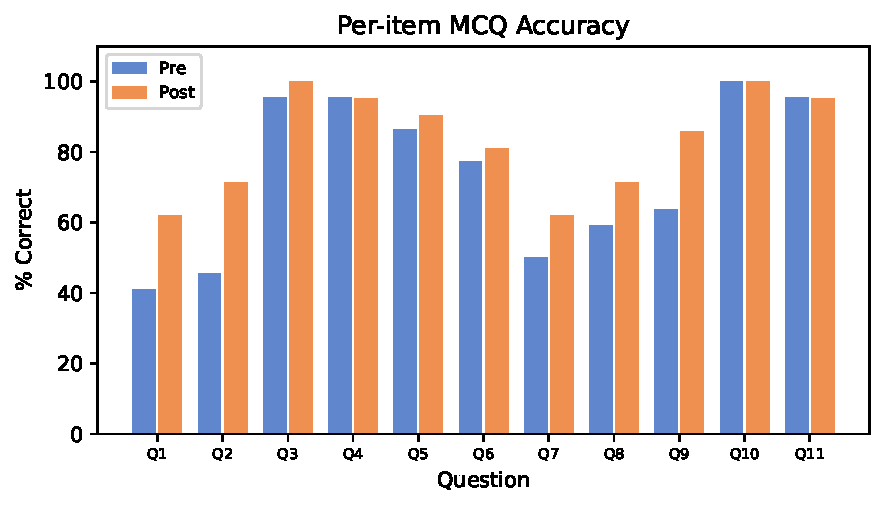
\includegraphics[width=\columnwidth]{figures/fig_mcq_peritem.pdf}
\caption{Per-item MCQ accuracy, pre vs.\ post. Largest gains on concepts directly practiced in the game.}
\label{fig:peritem}
\end{figure}

\subsubsection{Self-Confidence}

All four self-confidence items improved (Table~\ref{tab:confidence}), with the largest gain in ``analyzing test failures'' ($+0.38$, 7~improved, 0~declined).
Internal consistency was good (Cronbach $\alpha_{pre} = 0.811$, $\alpha_{post} = 0.839$).

\begin{table}[htbp]
\caption{Self-Confidence Shift ($N = 21$)}
\label{tab:confidence}
\centering
\small
\begin{tabular}{lcccc}
\toprule
Item & Pre & Post & $\Delta$ & $\uparrow/\!=\!/\!\downarrow$ \\
\midrule
Understand concepts & 3.43 & 3.57 & +0.14 & 3/16/2 \\
Write test case & 3.48 & 3.71 & +0.24 & 5/15/1 \\
Identify/debug errors & 3.48 & 3.67 & +0.19 & 4/15/2 \\
Analyze test failures & 3.24 & 3.62 & +0.38 & 7/14/0 \\
\bottomrule
\end{tabular}
\end{table}

\subsection{RQ2: Student Perception}

Table~\ref{tab:perception} summarizes post-session perception constructs.
Students rated the game highly across all dimensions, with 95\% agreeing it helped understand testing vs.\ debugging, 86\% finding it engaging, and 71\% preferring it over traditional lectures.
Cognitive load was moderate (3.19/5 for mental effort), and 71\% rated difficulty as appropriate.

\begin{table}[htbp]
\caption{Post-Session Perception ($N = 21$)}
\label{tab:perception}
\centering
\small
\begin{tabular}{lcc}
\toprule
Construct (items) & Mean & \% Agree \\
\midrule
Perceived Learning (4) & 4.06 & 86\% \\
Engagement (3) & 4.05 & 76\% \\
Usability (3) & 4.24 & 74\% \\
Cognitive Load (3) & 3.30 & --- \\
\bottomrule
\end{tabular}
\end{table}

Students most valued the interactive and immediate feedback aspects.
Representative comments include: \emph{``the code changing in real time demanding debugging,''} \emph{``the gamification,''} and \emph{``a game is always a good way to learn and engage people.''}
Main difficulties were Java syntax barriers (\emph{``the Java part was the toughest for me''}), debugging complexity, and initial game navigation confusion.
Table~\ref{tab:themes} summarizes the recurring themes from open-ended responses.

\begin{table}[htbp]
\caption{Thematic Analysis of Open-Ended Responses}
\label{tab:themes}
\centering
\small
\begin{tabular}{p{1.8cm}p{2.4cm}p{2.6cm}}
\toprule
Theme & Evidence & Interpretation \\
\midrule
Interactive Learning & \emph{``The gamification''}; feedback comments & Students valued active participation and immediate responses to testing actions \\
\addlinespace
Failure Awareness & \emph{``The code changing in real time demanding debugging''} & Students developed stronger understanding of software failures and the role of debugging \\
\addlinespace
Novelty \& Authenticity & \emph{``I never did testing before''} & The activity exposed students to practical testing experiences perceived as authentic \\
\addlinespace
Java Syntax Barrier & \emph{``The Java part was the toughest for me''} & Some challenges related to language proficiency rather than testing concepts \\
\addlinespace
Debugging Complexity & Comments on locating and repairing faults & Debugging remained cognitively demanding despite scaffolding mechanisms \\
\bottomrule
\end{tabular}
\end{table}

\subsection{RQ3: Behavioral Engagement (Telemetry)}

The game recorded 3,226~events from 22~active players (Table~\ref{tab:telemetry}).
Students with questionnaire matches averaged 46~minutes of active gameplay.

\begin{table}[htbp]
\caption{Sojourner Telemetry: Event Distribution ($N = 22$ players)}
\label{tab:telemetry}
\centering
\small
\begin{tabular}{p{2cm}p{3.5cm}r}
\toprule
Event Type & Meaning & Count \\
\midrule
Room unlocked & Player moved to a new level & 1,251 \\
Game progression & Room phase changed (e.g., talk $\to$ test $\to$ debug) & 404 \\
Conversation & Dialogue with robot companion completed & 304 \\
Test modified & Student edited test code in the editor & 272 \\
Test executed & Tests compiled and ran successfully & 211 \\
Test exec.\ failed & Compilation error or test assertion failed & 115 \\
Component fixed & Student correctly repaired sabotaged code & 100 \\
CUT modified & Student edited the class-under-test during debugging & 84 \\
Mutation detected & Student's tests caught the injected fault & 66 \\
Tests activated & Tests reached $\geq$50\% coverage and were set to monitor & 58 \\
Debug started & Sabotage detected; student entered debugging mode & 55 \\
Component destroyed & Sabotage went undetected; component damaged & 52 \\
Game started & Player logged in and began a session & 45 \\
Hidden test added & System provided a hint test after undetected sabotage & 34 \\
\midrule
\textbf{Total} & & \textbf{3,226} \\
\bottomrule
\end{tabular}
\end{table}

The progression funnel (Fig.~\ref{fig:funnel}) shows that all students started Room~1 (CryoSleep), 60\% reached Room~2, and progressively fewer advanced further; two students (8\%) completed all seven rooms.

\begin{figure}[htbp]
\centering
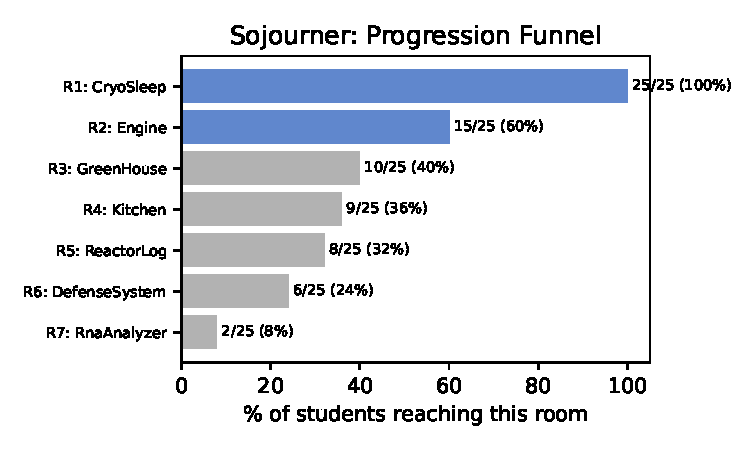
\includegraphics[width=\columnwidth]{figures/fig_progression_funnel.pdf}
\caption{Progression funnel: percentage of students reaching each room.}
\label{fig:funnel}
\end{figure}

The 52~\emph{ComponentDestroyedEvent}s indicate cases where students' tests failed to detect sabotage, triggering hidden tests as scaffolding (34~events).
This confirms the game's adaptive support mechanism was actively functioning.

An exploratory correlation analysis ($N = 14$ students with matched telemetry and questionnaire data) revealed a significant positive association between game progression and MCQ gains (Spearman $\rho = 0.633$, $p = 0.007$; Fig.~\ref{fig:correlation}).
Progression was also strongly correlated with test executions ($\rho = 0.860$, $p < 0.001$), confirming that advancement reflects genuine testing activity.

\begin{figure}[htbp]
\centering
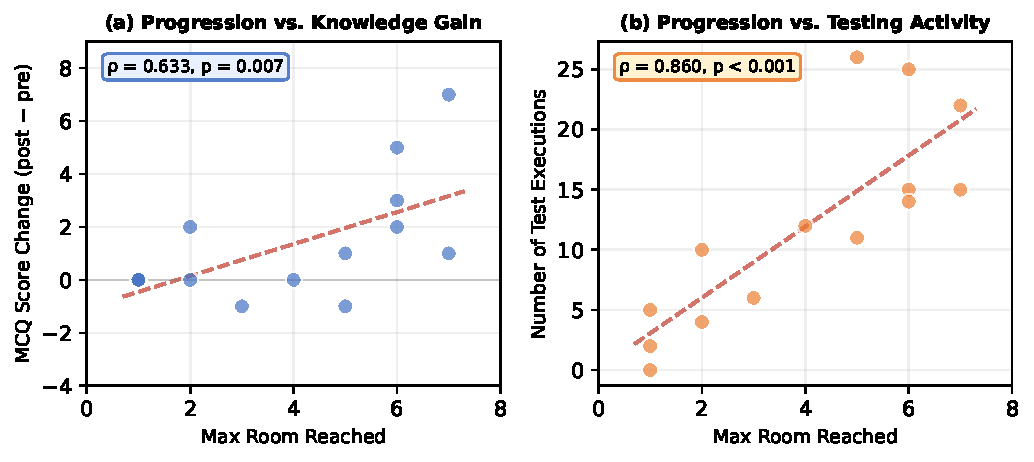
\includegraphics[width=\columnwidth]{figures/fig_correlation.pdf}
\caption{(a) Game progression vs.\ MCQ gains ($\rho = 0.633$, $p = 0.007$). (b) Progression vs.\ test executions ($\rho = 0.860$, $p < 0.001$).}
\label{fig:correlation}
\end{figure}

% ===========================================================================
\section{Discussion}
\label{sec:discussion}
% ===========================================================================

\subsection{Independent Replication and Extension}

Our findings extend the initial evaluation by Straubinger et al.~\cite{straubinger2025sojourner} to a different institutional and cultural context (Portuguese university, master's students).
The high engagement (86\%) and perceived learning (95\% for testing vs.\ debugging) are consistent with the original study's findings of over 80\% enjoyment, suggesting the game's effectiveness generalizes beyond its original setting.
Our study adds behavioral telemetry analysis---absent from the original evaluation---providing objective evidence that engagement correlates with learning.

\subsection{The Ceiling Effect}

The non-significant MCQ improvement ($p = 0.170$) should not be interpreted as ineffectiveness.
The pre-test mean of 8.3/11 (75\%) left limited room for improvement.
Sub-group analysis confirms that students who needed help most benefited most (normalized gain = 0.50 for low-baseline students).
Per-item analysis shows gains concentrated on concepts directly practiced in the game.
Future studies should use more challenging instruments calibrated to the target population.

\subsection{Behavioral Telemetry as Supporting Evidence}

Beyond the questionnaire-based findings, the game's telemetry provides objective behavioral evidence.
The significant correlation between progression and MCQ gains ($\rho = 0.633$, $p = 0.007$) provides evidence that the game's design---where advancement requires genuine testing and debugging skill---translates behavioral engagement into measurable learning.
The 34~hidden-test scaffolding events confirm that the game's adaptive support mechanism actively assisted struggling students, and the strong correlation between progression and test executions ($\rho = 0.860$) rules out passive navigation as an explanation.
This telemetry-based analysis demonstrates a practical advantage of game-based platforms over traditional exercises: built-in learning analytics that enable formative assessment without additional instrumentation.

\subsection{Qualitative Insights from Student Feedback}

Qualitative feedback revealed several recurring themes.
First, students valued the interactive nature of the game and the immediate feedback provided after testing and debugging actions.
Second, multiple participants highlighted that observing failures and repairing sabotaged components helped them better distinguish testing from debugging---reinforcing concepts that are often difficult to convey through traditional lectures alone.
Third, some students reported difficulties related to Java syntax and debugging complexity, suggesting that introductory scaffolding remains important when deploying the game with novice learners.
Overall, the qualitative findings complement the quantitative results by illustrating how students experienced the learning process and why they perceived the activity as engaging and educationally valuable.

\subsection{Equity Through Scaffolding}

Low-baseline students benefited most (normalized gain = 0.50 vs.\ 0.00 for high-baseline), suggesting that the game's scaffolding mechanisms---robot hints, hidden tests, progressive difficulty---provide support proportional to need.
Rather than uniformly improving all students, the game appeared particularly beneficial for students with lower initial knowledge, suggesting a compensatory or equity-enhancing effect.
This dimension is particularly relevant for heterogeneous classrooms where students enter with varying levels of prior knowledge.

\subsection{Practical Implications}

Based on our experience, we offer practical recommendations for instructors considering Sojourner under Sabotage:
\begin{itemize}
    \item Allow at least 70~minutes of gameplay; shorter sessions limit students to the tutorial level.
    \item Use the bulk account generation feature with participant codes matching questionnaire IDs for seamless data linkage.
    \item Brief students on Java/JUnit syntax before gameplay to reduce language-specific barriers.
    \item Use telemetry data for formative assessment: students with high compilation failure rates may need targeted support.
    \item Consider developing a lightweight monitoring dashboard to consume the game's JSON export; this significantly reduces the effort required to inspect student engagement patterns and supports evidence-based instructional decisions during and after the session.
\end{itemize}

% ===========================================================================
\section{Threats to Validity}
\label{sec:threats}
% ===========================================================================

\textbf{Internal validity.}
The single-group pre-test/post-test design without a control group limits causal interpretation.
The reuse of identical MCQ items in pre- and post-tests may introduce a testing effect, where participants' performance is influenced by prior exposure to the questions rather than actual conceptual improvement.
The ceiling effect in the Sojourner MCQ limits the observable range of improvement.

\textbf{Construct validity.}
The cognitive load items mix positive and negative valence (one item was reverse-coded), and the resulting scale showed poor internal consistency ($\alpha < 0$), suggesting that these items may not reliably measure a single construct.
Self-reported perception may not fully reflect actual learning.
Cognitive load findings should therefore be interpreted descriptively rather than as a validated construct score.

\textbf{External validity.}
The study was conducted with a single cohort ($N = 22$) at one institution, limiting the generalizability of findings to other populations or educational settings.
Despite these limitations, the study provides useful exploratory evidence about the educational potential of Sojourner under Sabotage, and the combination of knowledge questions, self-confidence items, perception constructs, and telemetry allows for a richer understanding of students' learning experience.

\textbf{Reliability.}
The sample size ($N = 22$) limits statistical power, and the correlation analysis ($N = 14$ matched students) is exploratory.
Cronbach's $\alpha$ values for self-confidence ($\geq 0.81$), perceived learning ($0.87$), and engagement ($0.75$) indicate acceptable to good internal consistency.

% ===========================================================================
\section{Conclusion}
\label{sec:conclusion}
% ===========================================================================

This paper presented an empirical evaluation of \emph{Sojourner under Sabotage} for teaching software testing and debugging to master's students.
The game produced high engagement (86\%), strong perceived learning (95\% for testing vs.\ debugging), and positive self-confidence shifts.
While MCQ gains were limited by a ceiling effect, sub-group analysis revealed that low-baseline students benefited substantially (normalized gain = 0.50).
Behavioral telemetry from 3,226 events further supported these findings, revealing a significant correlation between game progression and learning gains ($\rho = 0.633$, $p = 0.007$).

These results provide independent evidence that Sojourner under Sabotage is an effective and engaging tool for software testing education, with built-in telemetry enabling formative assessment.
Future work should evaluate the game in larger, multi-institutional studies with more discriminating knowledge instruments, and investigate long-term retention of testing skills.

\section*{Data Availability}
The replication package---including questionnaire data, in-game telemetry, and generated figures---is publicly available at: \url{https://github.com/aazaadef/Sojourner}

\section*{Acknowledgment}
This work was supported by FCT -- Funda\c{c}\~{a}o para a Ci\^{e}ncia e Tecnologia, I.P.\ by project reference UIDB/50008/2020 (DOI: \url{https://doi.org/10.54499/UIDB/50008/2020}) and by the doctoral grant PRT/BD/155023/2023.
The authors would also like to acknowledge the Promptme4Better project, funded by the European Union Erasmus+ Program and the Portugal National Agency under grant agreement number 2025-1-PT01-KA220-HED-000363565, and all partners involved in the project.
The authors used generative AI tools solely to support English language polishing and readability improvements.
All technical content, interpretations, and conclusions were created and verified by the authors, who take full responsibility for the final manuscript.

\balance
\bibliographystyle{IEEEtran}
\begin{thebibliography}{99}
\bibitem{straubinger2025sojourner} P.~Straubinger, T.~Greller, and G.~Fraser, ``Sojourner under Sabotage: A Serious Testing and Debugging Game,'' in \emph{Proc.\ FSE Companion '25}, ACM, 2025.
\bibitem{javamelody} JavaMelody, ``Open-source monitoring for Java applications,'' 2024. Available: https://github.com/javamelody/javamelody
\bibitem{garousi2020testing} V.~Garousi, A.~Rainer, P.~Lauv\aa{}s~Jr., and A.~Arcuri, ``Software-testing education: A systematic literature mapping,'' \emph{J.\ Syst.\ Softw.}, vol.~165, 2020.
\bibitem{straubinger2023survey} P.~Straubinger and G.~Fraser, ``A Survey on What Developers Think About Testing,'' in \emph{Proc.\ ISSRE '23}, IEEE, 2023, pp.~80--90.
\bibitem{mccauley2008debugging} R.~McCauley et~al., ``Debugging: a review of the literature from an educational perspective,'' \emph{Comput.\ Sci.\ Educ.}, vol.~18, no.~2, pp.~67--92, 2008.
\bibitem{jamil2016testing} M.~A.~Jamil et~al., ``Software Testing Techniques: A Literature Review,'' in \emph{Proc.\ ICT4M '16}, IEEE, 2016, pp.~177--182.
\bibitem{deterding2011gamification} S.~Deterding et~al., ``From game design elements to gamefulness: defining `gamification,'\,'' in \emph{Proc.\ MindTrek '11}, ACM, 2011, pp.~9--15.
\bibitem{blanco2023gamification} R.~Blanco et~al., ``Can gamification help in software testing education?'' \emph{J.\ Syst.\ Softw.}, vol.~200, 2023.
\bibitem{connolly2012systematic} T.~M.~Connolly et~al., ``A systematic literature review of empirical evidence on computer games and serious games,'' \emph{Comput.\ Educ.}, vol.~59, no.~2, pp.~661--686, 2012.
\bibitem{cooper2023serious} K.~M.~L.~Cooper, ``Introduction to Software Engineering for Games in Serious Contexts,'' in \emph{SE for Games in Serious Contexts}, Springer, 2023, pp.~1--16.
\bibitem{quintero2023serious} C.~A.~Caldas~Quintero and G.~A.~Cifuentes~\'{A}lvarez, ``Serious Games and Computer Programming Competencies Development,'' \emph{Rev.\ Iberoam.\ Tecnol.\ Aprendiz.}, vol.~18, no.~1, pp.~48--53, 2023.
\bibitem{fraser2019code} G.~Fraser et~al., ``Gamifying a Software Testing Course with Code Defenders,'' in \emph{Proc.\ SIGCSE '19}, ACM, 2019, pp.~571--577.
\bibitem{clegg2017teaching} B.~S.~Clegg, J.~M.~Rojas, and G.~Fraser, ``Teaching Software Testing Concepts Using a Mutation Testing Game,'' in \emph{Proc.\ ICSE-SEET '17}, IEEE, 2017, pp.~33--36.
\bibitem{valle2017testing} P.~H.~D.~Valle et~al., ``The Testing Game,'' in \emph{Proc.\ SBES '17}, 2017.
\bibitem{straubinger2024code} P.~Straubinger, L.~Bloch, and G.~Fraser, ``Engaging Young Learners with Testing Using Code Critters,'' in \emph{Proc.\ ICST '24 Workshops}, IEEE, 2024.
\bibitem{straubinger2023code} P.~Straubinger, L.~Caspari, and G.~Fraser, ``Code Critters: A Block-Based Testing Game,'' in \emph{Proc.\ ICST '23 Workshops}, IEEE, 2023, pp.~426--429.
\bibitem{lee2014gidget} M.~J.~Lee, ``Gidget: An online debugging game,'' in \emph{Proc.\ VL/HCC '14}, IEEE, 2014, pp.~193--194.
\bibitem{miljanovic2017robobug} M.~A.~Miljanovic and J.~S.~Bradbury, ``RoboBUG: A Serious Game for Learning Debugging,'' in \emph{Proc.\ ICER '17}, ACM, 2017, pp.~93--100.
\bibitem{li2019framework} C.~Li et~al., ``Towards a Framework for Teaching Debugging,'' in \emph{Proc.\ ACE '19}, ACM, 2019, pp.~79--86.
\bibitem{bonar1985preprogramming} J.~Bonar and E.~Soloway, ``Preprogramming Knowledge: A Major Source of Misconceptions in Novice Programmers,'' \emph{Hum.\ Comput.\ Interact.}, vol.~1, no.~2, pp.~133--161, 1985.
\bibitem{pea1986language} R.~D.~Pea, ``Language-independent conceptual `bugs' in novice programming,'' \emph{J.\ Educ.\ Comput.\ Res.}, vol.~2, no.~1, pp.~25--36, 1986.
\bibitem{kappen2013kaleidoscope} D.~L.~Kappen and L.~E.~Nacke, ``The kaleidoscope of effective gamification,'' in \emph{Proc.\ Gamification '13}, ACM, 2013, pp.~119--122.
\bibitem{toda2017dark} A.~M.~Toda et~al., ``The Dark Side of Gamification,'' in \emph{HEFA '17}, Springer, 2017, pp.~143--156.
\bibitem{kolb1984experiential} D.~A.~Kolb, \emph{Experiential Learning: Experience as the Source of Learning and Development}. Prentice-Hall, 1984.
\bibitem{hmelo2004problem} C.~E.~Hmelo-Silver, ``Problem-Based Learning: What and How Do Students Learn?'' \emph{Educ.\ Psychol.\ Rev.}, vol.~16, no.~3, pp.~235--266, 2004.
\bibitem{prince2004active} M.~Prince, ``Does Active Learning Work? A Review of the Research,'' \emph{J.\ Eng.\ Educ.}, vol.~93, no.~3, pp.~223--231, 2004.
\end{thebibliography}

\end{document}
